\section{Introduction}
\label{sec:intro}

% ============================== METHOD OVERVIEW (page 2) ==============================
\begin{figure*}[t]
\centering
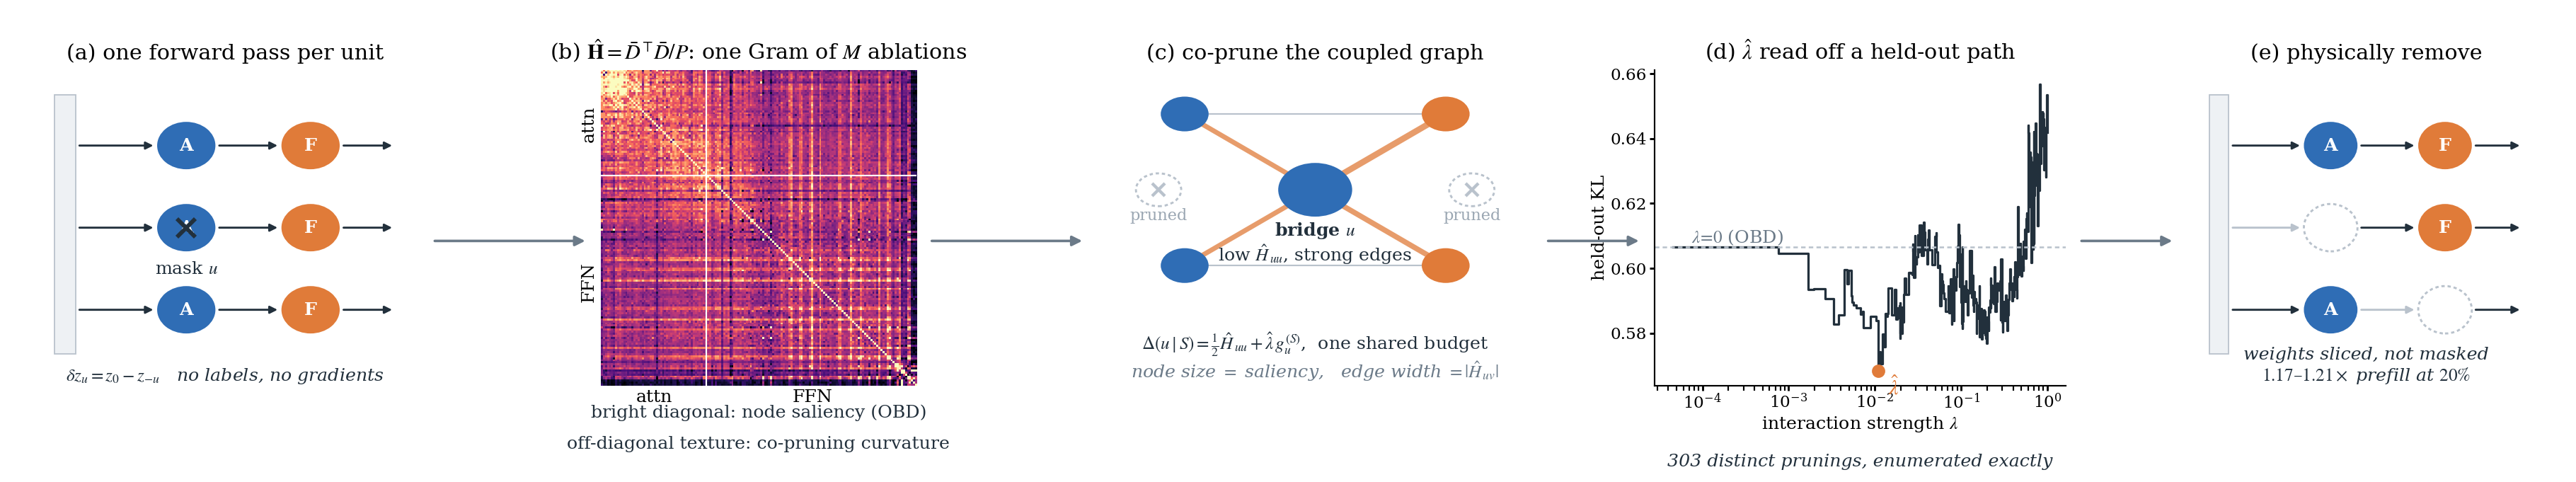
\includegraphics[width=\textwidth]{figs/fig_overview.png}
\caption{\textbf{Overview.} \textbf{(a)} One forward pass per removable unit records how the output
distribution moves when that unit alone is masked; no labels and no gradients. \textbf{(b)} The Gram
product of those $M$ features estimates the Fisher matrix of the pruning risk: its diagonal is classical
node saliency, its off-diagonal is co-pruning curvature. Shown is the measured curvature correlation on
Llama-3.1-8B-Instruct, units ordered attention-then-FFN. \textbf{(c)} One budgeted greedy on that
matrix, attention units and FFN groups drawing on a single budget; a low-saliency unit with strong
edges --- a \emph{bridge} --- is kept, because removing it alongside its partners is what costs.
\textbf{(d)} How far to trust the off-diagonal is measured rather than tuned: the family indexed by
$\lambda$ is finite, we enumerate its breakpoints exactly, and keep the member with the lowest held-out
KL. Shown is that path, all $303$ members of it, on the same model. \textbf{(e)} The mask is realised by
slicing weight matrices, so the speedup is measured on a smaller model and not on a masked one.}
\label{fig:overview}
\end{figure*}

Large language models (LLMs) deliver their capabilities at a parameter and latency cost that is prohibitive
for most deployments~\citep{vaswani2017attention,dubey2024llama3}. Structured pruning removes whole
computational units, such as attention heads and feed-forward (FFN) channel groups. It is the most
deployment-friendly route to compression: the pruned model stays dense and runs faster on commodity
hardware, without the specialized kernels that unstructured or semi-structured sparsity
needs~\citep{frantar2023sparsegpt,sun2024wanda}. The most practical setting is training-free, pruning
one-shot from a small unlabeled calibration set, which avoids the cost and the data dependence of
retraining~\citep{ma2023llmpruner,an2024flap}.

\textbf{The blind spot: nodes without edges.} Structured pruners score each removable unit and delete
the lowest-ranked ones, using weight~\citep{han2015learning},
activation~\citep{sun2024wanda,an2024flap} or local loss statistics~\citep{ma2023llmpruner,frantar2022obc}.
Ranking assumes that set-level damage is additive,
$\Delta\mathcal{L}(S)\approx\sum_{u\in S}\Delta\mathcal{L}(u)$. In a Transformer it is not. Attention
and FFN units read and write one shared residual stream, so pruning is a joint operation on a coupled
system: two units that look weak alone can be jointly indispensable, and two salient-looking ones can
be partly redundant when their perturbations overlap. A ranking is blind to this even when attention
and FFN units share a single global order, and it will delete a low-saliency \emph{bridge} unit
together with the units that depend on it. The interaction has to be modeled. \emph{Prune the edges,
not just the nodes.}

\textbf{One matrix, read two ways.} Interactions could be added heuristically --- by correlating
activations, say --- but that measures the wrong thing, and not by a little. Activation correlation is a
property of a layer's inputs; pruning dependence is a property of how two removals \emph{jointly} move
the model's output. Nothing in the former refers to the output at all, and two perfectly correlated
units may be jointly harmless, because each covers for the other, or jointly critical, because whatever
consumes them needs both --- the correlation is identical in the two cases. An interaction term worth
having must therefore be derived from the quantity being protected, so we derive it from the pruning
objective. Define
pruning risk as the token-level KL divergence between the frozen model and its masked copy over
unlabeled text. The masked model equals the frozen one at zero pruning, so both the value and the
gradient of this risk vanish there, and the local expansion begins at second order as a quadratic form
$\tfrac12 s^\top \Hmat s$ in the structured mask $s$. That single matrix has a direct reading
(\cref{fig:overview}):
\begin{center}
\emph{its diagonal $\Hmat_{uu}$ is classical node saliency; its off-diagonal $\Hmat_{uv}$ is a
\textbf{co-pruning curvature edge}, the mixed curvature governing the predicted marginal risk of
removing $u$ and $v$ together.}
\end{center}
These are not hand-designed information-flow arrows but symmetric interactions in the same Fisher
geometry that defines the saliency, spanning attention$\leftrightarrow$FFN pairs across all layers.
Pruning becomes global co-pruning-risk minimisation rather than node ranking, and it inherits a
classical floor: dropping the off-diagonal recovers an Optimal-Brain-Damage
saliency~\citep{lecun1989obd,hassibi1993obs} lifted to structured units, so \method is its
cross-module generalisation.

\textbf{Why the off-diagonal is affordable.} Ablate each removable unit once and record how the output
distribution moves. The inner product of two such recorded shifts estimates the curvature entry for
that pair, so the full $M\times M$ estimator is a Gram product of $M$ ablations rather than $O(M^2)$
pairwise sweeps, and no gradient is ever taken. Units are then removed greedily under one shared
budget, each candidate charged its own cost plus its accumulated interaction with what has already
gone, so the attention-versus-FFN split follows from the objective instead of being fixed by hand.
Ablations replace the derivative columns, and \cref{app:th-est} measures what that substitution costs.
Nothing is trained. The one quantity that must be chosen, how far to
trust the pairwise term, is measured rather than tuned: it indexes a family of prunings that is finite
and whose breakpoints we enumerate exactly, in the spirit of LARS~\citep{efron2004lars}, and we keep
the member with the lowest held-out risk, consulting no labels and no benchmarks.

\textbf{What this buys.} We evaluate five dense LLMs from $3$B to $24$B across the Llama-3, Falcon3 and
Mistral lineages against seven training-free baselines, under one shared guard and harness, on three
language-modelling corpora and twelve multiple-choice benchmarks scored on their full test sets at
five ratios from $10\%$ to $50\%$, all five of them on Mistral-Small-24B. Against the per-column best of every baseline --- an
envelope, not one competitor --- \method takes $70$ of the $105$ cells this grid contains: $38$ of the
$45$ perplexity cells and $32$ of the $60$ capability-group cells. Nothing in the construction is
specific to a decoder-only stack: pointed at \vlmGridModelsW\ vision--language models, where the unit
inventory spans two towers and one budget is shared across both, the same estimator and the same
selector lead every training-free baseline on all \vlmNcolsW\ headline columns
(\cref{sec:exp-vlm}). The edge term also acts through a population we can name and
delete on demand. Low-saliency, high-connectivity \emph{bridge} units are what node-first scoring
removes first; forcing them out, against a control matched unit-for-unit on saliency, unit type and
cost and completed by the same shared fill, costs nineteen of twenty capability-group cells across
five models, by up to $23.7$ points --- while on three of the five perplexity moves the other way. Given one budget and no per-type rule, the same objective independently arrives at the
same allocation across five models and five ratios: the first half of a network's depth pruned
entirely out of FFN width, attention touched only beyond it, in thirteen of the seventeen solutions
that remove any attention at all --- and eight of the twenty-five solutions, on two of the models,
remove none anywhere.
